\section{Canton Ticino}
\subsection{La politica di comunicazione istituzionale tramite i social media.}
L’amministrazione cantonale è presente sui social media, in quanto l’attività dei media tradizionali è in forte calo in rapporto alle piattaforme digitali e quindi è necessario essere attivi anche in questo ambito in modo tale da riuscire a raggiungere più persone. Inoltre, gli studi effettuati dall’istituto fög dell’Università di Zurigo\footnote{Repubblica e Cantone Ticino, “Social media, Rapporto annuale 2017”, Bellinzona, 2018, consultato l’11.01.2019} evidenziano che sommando i follower dei profili dell’amministrazione cantonale sono 25500 utenti. Su ogni piattaforma il numero è in aumento, per esempio su Facebook c’è stato un incremento del 46\% rispetto al 2016 mentre su Twitter addirittura del 340\%. Essa è presente con il proprio nome solamente su Youtube con un canale. Per il resto non è presente esplicitamente su gli altri social media, ma “delega” ad altre pagine più specifiche la comunicazione online di quel tema.Per esempio su Facebook sono presenti le Biblioteche, la polizia, gioventù e sport, ecc. mentre su Twitter troviamo l’ufficio della statistica del Canton Ticino. 
\newpage
\subsection{Quali social utilizza e come li utilizza (osservazioni personali e analisi comunicazione istituzionale)}
\textbf{Facebook.}\\
La comunicazione istituzionale tramite social media viene effettuata principalmente tramite Facebbok e Twitter. Sul primo è presente la pagina del sistema bibliotecario ticinese, su questa pagina sono stati presi in analisi: 
\begin{itemize}
    \item L’utente medio
    \item L’evoluzione dei “mi piace”
    \item Le visualizzazioni di pagina
    \item La copertura dei post
\end{itemize}
Il primo punto riguarda le generalità degli utenti che frequentano la pagina. In questo modo si è in grado di pubblicare dei post più efficaci in quanto si conoscono il sesso, l’età, la nazionalità, la residenza e la lingua madre. Il secondo punto che è stato analizzato riguarda l’evoluzione dei “mi piace” dei post della pagina.
\begin{figure}[h]
        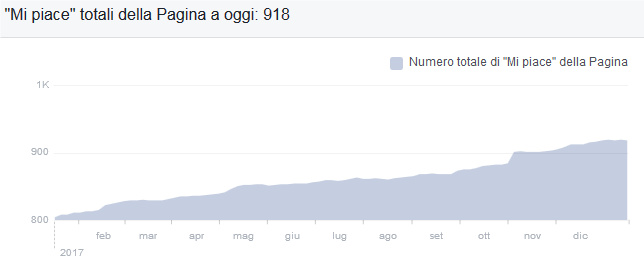
\includegraphics[width=\textwidth]{capitoli/foto/like.png}
        \caption {-Evoluzione dei "mi piace" sulla pagina del sistema bibliotecario ticinese, (Fonte: Repubblica e Cantone Ticino, "Social media, Rapporto annuale 2017", Bellinzona, 2018)}
        \label{fig:my_label}
\end{figure}

Come si può vedere dal grafico, i “mi piace” complessivi della pagina sono in costante aumento. Da 804 a 918, e questi equivalgono al 14,2 \% rispetto al 2016 . Questo aumento è dovuto soprattutto all’aumento di persone che utilizzano i social media, la pagina del sistema bibliotecario pubblica dei post con le promozioni o degli eventi che sono presenti presso le varie biblioteche ticinesi. In questo modo se un’utente è interessato a queste proposte metterà “mi piace” al post. Il terzo punto riguarda il numero totali di visualizzazioni della pagina e il quarto punto spiega la copertura dei post, ovvero il numero di persone a cui i post sono stati mostrati.
\newpage
\textbf {Twitter}\\
Invece su Twitter, il Consiglio di stato ha un profilo ufficiale. La pagina conta 1027 followers . Le reazioni ai tweet sono poche, infatti sia i like che i retweet sono pochissimi rispetto alle persone che seguono il profilo. Da quando Il Consiglio di Sato ha deciso di utilizzare questa piattaforma come ulteriore strumento di comunicazione, ovvero dal 2014, sono stati pubblicati 4167 tweet, si può quindi dire che sono attivi nella pubblicazioni di informazioni. Anche per questo social media sono stati effettuate delle analisi più approfondite. In particolare sulla pagina della polizia cantonale. Come per Facebook, sono stati presi in considerazione:
\begin{itemize}
    \item L’utente medio
    \item L’evoluzione dei “mi piace”
    \item Le visualizzazioni di pagina
    \item La copertura dei post
\end{itemize}
\begin{figure}[h]
    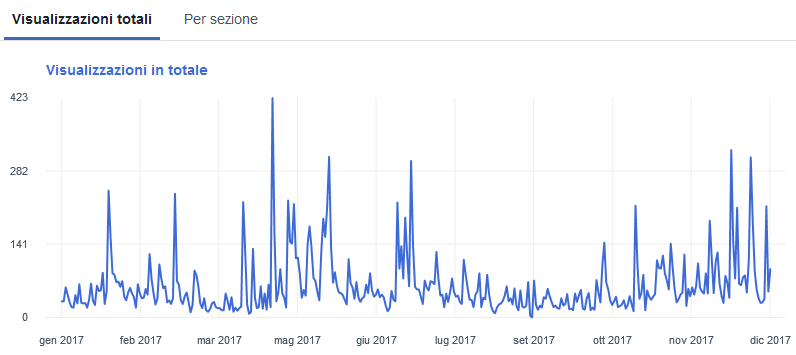
\includegraphics[width=\textwidth]{capitoli/foto/visualizzazioni.png}
    \caption{-Visualizzazioni di pagina sulla pagina della polizia cantonale, (Fonte: Repubblica e Cantone Ticino, "Social media, Rapporto annuale 2017", Bellinzona, 2018}
    \label{fig:my_label}
\end{figure}

Come si può leggere dal grafico le visualizzazioni della pagina sono stati regolari, ma bisogna segnalare alcuni picchi casuali come in Aprile quando vennero toccate le 423 visualizzazioni. Su questa pagina Twitter vengono pubblicate tutte le informazioni rigardanti gli interventi della polizia oppure le notizie riguardanti il traffico o dei possibili incidenti in Ticino.
Un social media in ascesa è sicuramente Youtube, questa piattaforma permette di caricare video tramite un canale, cosa che il Canton Ticino possiede. Per essere efficaci su Youtube bisogna essere costanti nel caricare contenuti interessanti per gli utenti e magari per attirare nuovi spettatori. In questo caso, la comunicazione istituzionale del canton Ticino potrebbe essere migliorata, dato che vengono pubblicati pochi video ed tra di essi passa molto tempo e soprattutto le reazioni degli utenti ai video sono molto poche, sia i like che i commenti. Di conseguenza non ci sono neanche discussioni sotto i video e questo è un peccato dato  che tramite la politica si potrebbero sviluppare dei dibattiti anche molto accessi che porterebbero visibilità al canale e di conseguenza al Consiglio di Stato in generale.  Questo social media potrebbe essere sfruttato meglio dalla nostra comunicazione istituzionale. Inoltre un vantaggio di questo mezzo comunicativo è che tramite dei video può risultare più semplice spiegare dei concetti politici rispetto a dei post su altre piattaforme, quali Twitter, Facebook e Instagram. Ad esempio per le votazioni del 25.11.2018 in merito all’iniziativa dell’autodeterminazione o al referendum il cui tema era la base legale per la sorveglianza degli assicurati(LPGA)  avrebbero potuto sfruttare i video e il loro canale per pubblicare dei contenuti che spiegassero bene e nel dettaglio i temi e magari esporre la posizione del Consiglio di stato in merito. Un social media che negli ultimi anni sta prendendo il sopravvento sugli altri è sicuramente Instagram. I numeri di questa piattaforma sono cresciute in modo esponenziale soprattutto tra i giovani e per una comunicazione politica che vuole coinvolgere più fasce d’età possibile porterebbe comunque molta visibilità. Il Consiglio di Stato non è ancora presente su questo mezzo di comunicazione. L’apertura di una pagina con lo stesso scopo di quella di Twitter porterebbe solo vantaggi alla comunicazione istituzionale del canton Ticino. Inizialmente sarebbe difficile riuscire ad imporsi anche su questa piattaforma, ma tramite la costanza nella pubblicazione dei post e tenendo in considerazione la grande quantità di persone che utilizzano questa piattaforma potrebbe portare grande visibilità alla comunnicazione istituzionale del Canton Ticino.
\subsection{Uso dei social media da parte del partito PPD in Ticino.}
Fabio Bacchetta-Cattori, in merito alla comunicazione del suo partito, ha detto che negli ultimi 2-3 anni sono stati fatti passi avanti, soprattutto grazie al nuovo segretario che è Nicolò Parente. In generale, questo sviluppo è stato molto positivo dato che l’ha trovato non troppo eccessivo ed espansivo, anche se alcuni membri del partito secondo lui hanno un utilizzo dei social media molto giovanile. Il partito è presente sui social media su Facebook, Twitter, Youtube e Instagram. Sono attivi soprattutto su Facebook e Twitter che sono stati i primi due mezzi comunicativi in cui il PPD Ticino ha creato un proprio profilo. Ambedue nel 2009 . In entrambi i casi vengono pubblicati dei post in cui si capisce l’opinione del partito. Ad esempio, come si vede nell’immagine, è stato pubblicato questo contenuto, dove veniva promossa l’iniziativa che stava sostenendo il PPD Ticino. Inoltre bisogna sottolineare che c’è stata una risposta ad un commento lasciato da un utente che esprimeva le proprie perplessità sulla proposta. Tale aspetto non è assolutamente da sottovalutare, dato che in questo modo le persone percepiscono la volontà del partito nel risolvere i problemi o i disagi dei cittadini. Mostrandosi disponibili nel fornire delle spiegazioni in maniera diretta ed esaustiva come è successo in questa occasione è il miglior modo per incrementare la propria visibilità sui social media e poi per ricevere degli apprezzamenti per la disponibilità e la professionalità dimostrata.

\begin{figure}[h!]
    \centering
    
\includegraphics[width=0.4\textwidth]{capitoli/foto/PPD.png}
    \caption{-Post sull’iniziativa del PPD dello stop nell’incremento dei premi dell’assicurazione, (Fonte: Pagina del PPD Ticino su Facebook), Bellinzona, 2018}
    \label{fig:my_label}
\end{figure}

Per quanto riguarda gli altri due social media, ovvero Youtube e Instagram vengono utilizzati molto meno. Il primo ha tre video caricati da quando è stato aperto, quindi il 24 aprile 2018  e i temi dei contenuti che sono stati caricati riguardano l’iniziativa che ha sostenuto il partito. Invece per Instagram si hanno pochi dati e soprattutto pochi post, i quali sono di augurio di buon anno oppure buone feste.
Personalmente penso che il PPD Ticino si muove abbastanza bene sui social media, soprattutto su Twitter e Facebook dove tiene il proprio profilo aggiornato tramite la pubblicazione di nuovi contenuti a scadenza regolare. Questo è un aspetto molto importante, dato che gli utenti che seguono la pagina non perdano interesse.  L’uso di Youtube risulta interessante, in quanto i video che vengono caricati servono a spiegare o rafforzare un pensiero del partito. Potrebbe essere pubblicizzato un po’ di più tramite gli altri social media, in modo tale da incuriosire le persone a guardare i contenuti del canale e magari iniziare a seguirlo con più frequenza. Invece per il momento il profilo Instagram potrebbe essere sviluppato e quindi reso più attraente per gli utenti interessati alle idee del partito. Ad esempio tramite la pubblicazione costante di contenuti che siano in grado di coinvolgere i giovani che frequentano questa piattaforma Di conseguenza non si può affermare se il profilo del PPD Ticino è efficace o meno, bensì che con degli accorgimenti potrebbe diventare una risorsa fondamentale per la comunicazione tramite i social media del partito.

\subsection{Osservazioni personali e analisi comunicazione istituzionale}
Per Paolo Beltraminelli in Ticino si è un po’ indietro nell’utilizzo dei social media in ambito politico anche se negli utili anni sono stati fatti dei passi avanti. Per esempio si è compreso che per riuscire ad attirare i giovani alla politica serve parlare su degli argomenti ben precisi rispetto che sulle ideologie dei diversi partiti. Di conseguenza anche i movimenti politici devono essere in grado di focalizzarsi su uno o più temi ben definiti e pubblicare in continuazione dei post tramite i propri profili. In modo tale da tenere informati gli utenti che ti seguono. Inoltre in questo modo si può “fidelizzare” le persone che ti seguono, dato che essendo interessati ad uno tema controlleranno sul profilo istituzionale se ci sono ulteriori informazioni.
Entrambi i politici ritengono che la comunicazione istituzionale tramite i social media è rimasta un po' attardata ma riconoscono comunque che il tentativo di utilizzare questi potenti strumenti comunicativi regolarmente e in maniera efficace. 
Secondo me il Canton Ticino sfrutta abbastanza bene questi metodi comunicativi, in particolare Twitter e Facebook dove vengono pubblicati dei post regolarmente e con lo scopo di informare gli utenti. Però se si ha lo scopo di attirare un numero di persone elevato potrebbero essere meno diplomatici nella pubblicazione di alcuni contenuti, per esempio il tema dei migranti potrebbe essere sfruttato per attirare una grossa quantità di utilizzatori dei social media, in modo tale da creare dei dibattiti sotto i post o i tweet. Così facendo, gli elettori interessati a dire la propria opinione o a ribattere a un’opinione contraria alla loro sarebbero invogliati a farlo. In questo modo, le pagine gestite dal Cantone aumenterebbero di visibilità e ovviamente tutto ciò, sarebbe positivo per migliorare o addirittura rafforzare l’immagine che la popolazione ha nei confronti dell’assemblea ticinese. Potrebbero essere sfruttati maggiormente Youtube e Instagram. Il primo per spiegare con dei video dei temi importanti che potrebbero riguardare le votazioni. Un metodo sarebbe quello di sponsorizzare il proprio canale tramite dei post sugli altri social media. Ad esempio, pubblicare un post su Facebook o Twitter in cui si informano gli utenti di quelle piattaforme, che sul canale Youtube del Canton Ticino è stato caricato un video, con una spiegazione su un tema di attualità. Dovrà essere presente il link del canale, in modo da semplificare il passaggio da un social media all’altro. Per quanto riguarda Instagram, penso che sia il più complicato da utilizzare in ambito politico, perché è utilizzato soprattutto da persone giovani e quindi risulta complicato avvicinarli a questo mondo. Per di più su questo strumento comunicativo sono più efficaci le foto o i video rispetto a dei testi argomentati come potrebbero essere più idonei su un media più tradizionale come un giornale. È quindi compito del politico o dell’ente istituzionale pensare, creare e poi pubblicare dei contenuti che si avvicinano alla realtà giovanile. Bisogna anche sottolineare che su Instagram è molto difficile riscontrare successo come istituzione, dato che gli utenti non possono identificarsi in una persona fisica come succede nel caso di Salvini, che grazie anche alle stories riesce a creare un contatto “diretto” con i propri follower.

